\documentclass[11pt,oneside]{book}

\usepackage[a4paper,margin=2.2cm]{geometry}
\usepackage{xcolor}
\usepackage{hyperref}
\usepackage{tikz}
\usepackage{listings}
\usepackage{array}
\usepackage{longtable}
\usepackage{float}

\usetikzlibrary{arrows.meta,positioning,shapes.geometric,shapes.misc,calc,fit}

\definecolor{bookblue}{HTML}{0A4A66}
\definecolor{bookteal}{HTML}{2A9D8F}
\definecolor{bookgold}{HTML}{D17C1D}
\definecolor{booksand}{HTML}{F4EFE6}
\definecolor{bookgray}{HTML}{4D5562}
\definecolor{bookred}{HTML}{B85042}
\definecolor{codebg}{HTML}{FBF7F0}

\hypersetup{
  colorlinks=true,
  linkcolor=bookblue,
  urlcolor=bookteal,
  citecolor=bookblue,
  pdftitle={Project Structure Book},
  pdfauthor={Soroosh AGHAEI}
}

\setlength{\parindent}{0pt}
\setlength{\parskip}{0.55em}
\renewcommand{\arraystretch}{1.15}

\lstdefinestyle{bookcode}{
  backgroundcolor=\color{codebg},
  basicstyle=\ttfamily\small,
  frame=single,
  rulecolor=\color{bookgray!35},
  keywordstyle=\color{bookblue},
  commentstyle=\color{bookteal!80!black},
  stringstyle=\color{bookgold!80!black},
  showstringspaces=false,
  keepspaces=true,
  columns=fullflexible,
  breaklines=true
}

\lstdefinelanguage{yaml}{
  morekeywords={true,false,null},
  sensitive=false,
  morecomment=[l]{\#},
  morestring=[b]",
  morestring=[b]'
}

\newcommand{\memorybox}[1]{
  \begin{center}
    \setlength{\fboxsep}{8pt}
    \fcolorbox{bookteal}{booksand}{\parbox{0.92\linewidth}{#1}}
  \end{center}
}

\newcommand{\actionbox}[1]{
  \begin{center}
    \setlength{\fboxsep}{8pt}
    \fcolorbox{bookblue}{bookblue!5}{\parbox{0.92\linewidth}{#1}}
  \end{center}
}

\title{\textbf{Project Structure Book}\\[0.5em]\large using the \texttt{py\_engine\_room} example layout}
\author{Soroosh AGHAEI}
\date{March 11, 2026}

\begin{document}

\maketitle
\tableofcontents

\chapter{How To Use This Book}

This book is a standalone guide to project structure design. It uses \texttt{py\_engine\_room} as a worked example, but the patterns are meant to transfer to many project types.  
It covers:
\begin{itemize}
  \item root setup and governance files,
  \item reusable templates for different project families,
  \item runnable examples that prove the patterns,
  \item data and output boundaries,
  \item automation tools,
  \item notebook and learning workflows.
\end{itemize}

The goal is simple: after reading it, you should be able to design, review, or refactor a project structure without depending on hidden context or tribal knowledge.

\memorybox{
\textbf{Working rule:} treat every folder and file in this book as a design choice with a reason.  
If you cannot explain why a path exists, the structure is not finished yet.
}

\actionbox{
\textbf{Recommended reading order}
\begin{itemize}
  \item Start with the foundation rules and the visual model.
  \item Learn the root map and the default readable project tree.
  \item Study the file-writing and pipeline chapters.
  \item Compare the application, library, and research shapes.
  \item Finish with the build-from-zero, maintenance, and review chapters.
\end{itemize}
}

\begin{figure}[H]
\centering
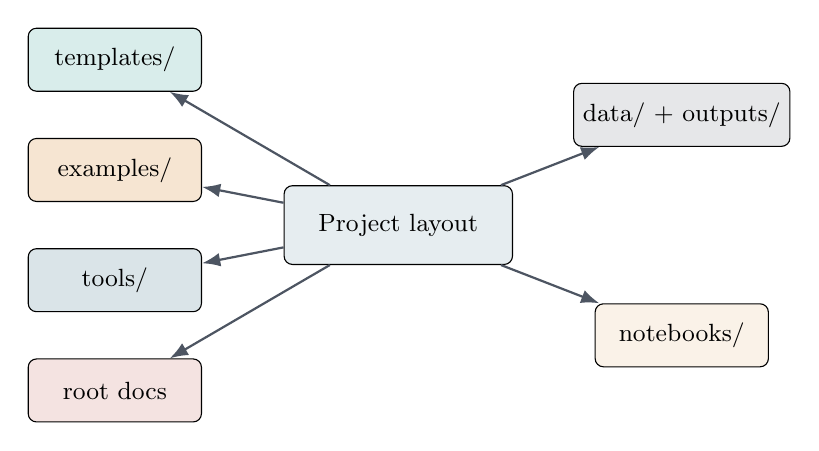
\begin{tikzpicture}[>=Latex, every node/.style={font=\small}]
  \node[draw, rounded corners=3pt, fill=bookblue!10, minimum width=2.9cm, minimum height=1.0cm] (root) at (0,0) {Project layout};
  \node[draw, rounded corners=3pt, fill=bookteal!18, minimum width=2.2cm, minimum height=0.8cm] (templates) at (-3.6,2.1) {templates/};
  \node[draw, rounded corners=3pt, fill=bookgold!20, minimum width=2.2cm, minimum height=0.8cm] (examples) at (-3.6,0.7) {examples/};
  \node[draw, rounded corners=3pt, fill=bookblue!15, minimum width=2.2cm, minimum height=0.8cm] (tools) at (-3.6,-0.7) {tools/};
  \node[draw, rounded corners=3pt, fill=bookred!16, minimum width=2.2cm, minimum height=0.8cm] (docs) at (-3.6,-2.1) {root docs};
  \node[draw, rounded corners=3pt, fill=bookgray!14, minimum width=2.2cm, minimum height=0.8cm] (data) at (3.6,1.4) {data/ + outputs/};
  \node[draw, rounded corners=3pt, fill=bookgold!10, minimum width=2.2cm, minimum height=0.8cm] (nb) at (3.6,-1.4) {notebooks/};

  \draw[->, thick, bookgray] (root) -- (templates);
  \draw[->, thick, bookgray] (root) -- (examples);
  \draw[->, thick, bookgray] (root) -- (tools);
  \draw[->, thick, bookgray] (root) -- (docs);
  \draw[->, thick, bookgray] (root) -- (data);
  \draw[->, thick, bookgray] (root) -- (nb);
\end{tikzpicture}
\caption{Example layout used throughout the book.}
\end{figure}

\chapter{Design Principles}

Before choosing folders and files, you need a small set of design rules.  
Without these rules, even a project that looks organized at first can become hard to read after a few weeks.

\section*{What Readability Actually Means}

A readable project lets a new contributor answer the basic engineering questions quickly:
\begin{itemize}
  \item Where does execution start?
  \item Where is the reusable logic?
  \item Which values come from configuration?
  \item Which files are generated outputs rather than source?
  \item Which tests prove the important behavior?
\end{itemize}

If those answers are slow or ambiguous, the structure is not readable, even if the folder names look tidy.

\begin{figure}[H]
\centering
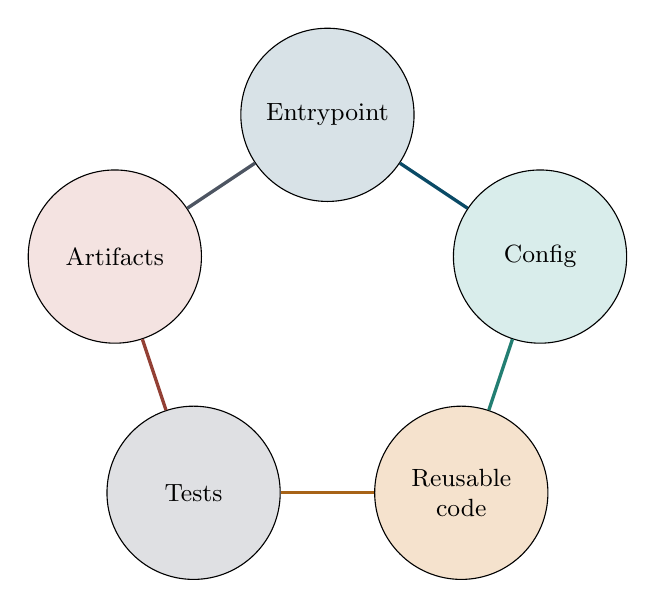
\begin{tikzpicture}[>=Latex, every node/.style={font=\small, align=center}]
  \node[draw, circle, fill=bookblue!16, minimum size=2.2cm] (entry) at (0,2.6) {Entrypoint};
  \node[draw, circle, fill=bookteal!18, minimum size=2.2cm] (config) at (2.7,0.8) {Config};
  \node[draw, circle, fill=bookgold!22, minimum size=2.2cm] (code) at (1.7,-2.2) {Reusable\\code};
  \node[draw, circle, fill=bookgray!18, minimum size=2.2cm] (tests) at (-1.7,-2.2) {Tests};
  \node[draw, circle, fill=bookred!16, minimum size=2.2cm] (art) at (-2.7,0.8) {Artifacts};

  \draw[very thick, bookblue] (entry) -- (config);
  \draw[very thick, bookteal!80!black] (config) -- (code);
  \draw[very thick, bookgold!80!black] (code) -- (tests);
  \draw[very thick, bookred!80!black] (tests) -- (art);
  \draw[very thick, bookgray] (art) -- (entry);
\end{tikzpicture}
\caption{A healthy project keeps five ideas separate: entrypoint, configuration, reusable code, tests, and produced artifacts.}
\end{figure}

\section*{The Seven Rules To Memorize}

\begin{enumerate}
  \item Keep the entrypoint thin.
  \item Put reusable logic under \texttt{src/}.
  \item Load configuration once and pass structured values forward.
  \item Keep mutable data and outputs out of source folders.
  \item Make tests verify the behavior users actually depend on.
  \item Keep the public API small and intentional.
  \item Add folders only when they own a real responsibility.
\end{enumerate}

\memorybox{
\textbf{The shortest reliable summary:} source code explains logic, configuration explains variation, tests explain trust, and outputs explain what happened during a run.
}

\section*{What Usually Goes Wrong}

Many weak projects do not fail because the code is impossible.  
They fail because structure slowly stops telling the truth.

\begin{lstlisting}[style=bookcode]
messy_project/
  final_script.py
  final_script_v2.py
  helpers.py
  utils.py
  data.csv
  output_final.txt
  test_new.py
  notebook_fixed.ipynb
\end{lstlisting}

This kind of tree creates immediate problems:
\begin{itemize}
  \item \texttt{helpers.py} and \texttt{utils.py} say nothing about responsibility.
  \item multiple root scripts compete to be the true entrypoint.
  \item data, source, outputs, and experiments all live together.
  \item names like \texttt{final\_script\_v2.py} encode confusion instead of design.
\end{itemize}

\section*{Naming Rules That Protect Readability}

Naming is structural, not cosmetic.  
Good names reduce the need for explanation because they reveal role directly.

Recommended defaults:
\begin{itemize}
  \item package names: lower snake case, for example \texttt{my\_project},
  \item modules: named after responsibility,
  \item example module names: \texttt{config.py}, \texttt{pipeline.py}, \texttt{logging\_utils.py},
  \item tests: name after the behavior they verify, for example \texttt{test\_import.py},
  \item output directories: derived from run name or date, not vague labels like \texttt{new/} or \texttt{final/}.
\end{itemize}

Avoid names like \texttt{misc}, \texttt{utils}, \texttt{temp}, or \texttt{stuff}.  
Those names usually mean the design decision has not been made yet.

\section*{When A New Folder Is Justified}

A new folder is usually justified only if at least one of these is true:
\begin{itemize}
  \item it contains a group of files with one shared responsibility,
  \item it separates mutable state from stable source code,
  \item it creates a clear boundary for imports, tests, or tooling,
  \item it reduces confusion for a new contributor.
\end{itemize}

If a folder exists only because the repository felt empty, it should not exist.

\actionbox{
\textbf{Top-level folder test}
\begin{itemize}
  \item Can you explain the folder in one sentence?
  \item Would the sentence be different from the sentence for every other top-level folder?
  \item Does the folder reduce confusion rather than merely spread files around?
\end{itemize}
}

\chapter{Visual Model}

\section*{Core Top-Level Shape}
\begin{figure}[H]
\centering
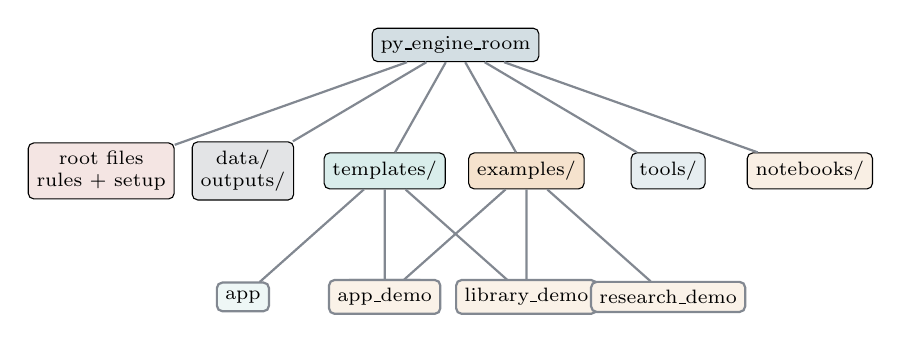
\begin{tikzpicture}[
  level distance=16mm,
  sibling distance=18mm,
  edge from parent/.style={draw=bookgray!70, thick},
  every node/.style={font=\scriptsize, draw, rounded corners=2pt, align=center, inner sep=3pt}
]
\node[fill=bookblue!18]{py\_engine\_room}
  child { node[fill=bookred!15]{root files\\rules + setup} }
  child { node[fill=bookgray!16]{data/\\outputs/} }
  child { node[fill=bookteal!18]{templates/}
    child { node[fill=bookteal!8]{app} }
    child { node[fill=bookteal!8]{library} }
    child { node[fill=bookteal!8]{research} }
  }
  child { node[fill=bookgold!22]{examples/}
    child { node[fill=bookgold!10]{app\_demo} }
    child { node[fill=bookgold!10]{library\_demo} }
    child { node[fill=bookgold!10]{research\_demo} }
  }
  child { node[fill=bookblue!10]{tools/} }
  child { node[fill=bookgold!12]{notebooks/} };
\end{tikzpicture}
\caption{Mental map of a reusable project structure with clear teaching, execution, and boundary zones.}
\end{figure}

\section*{Pipeline Shape For Most Projects}
\begin{figure}[H]
\centering
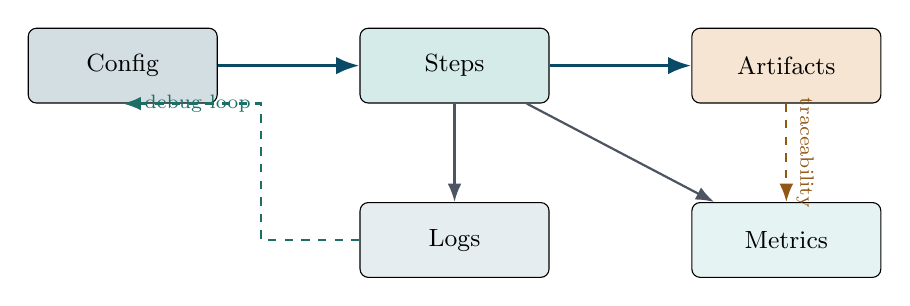
\begin{tikzpicture}[>=Latex, node distance=1.8cm, every node/.style={font=\small}]
  \node[draw, rounded corners=3pt, fill=bookblue!18, minimum width=2.4cm, minimum height=0.95cm] (cfg) {Config};
  \node[draw, rounded corners=3pt, fill=bookteal!20, minimum width=2.4cm, minimum height=0.95cm, right=of cfg] (steps) {Steps};
  \node[draw, rounded corners=3pt, fill=bookgold!20, minimum width=2.4cm, minimum height=0.95cm, right=of steps] (art) {Artifacts};
  \node[draw, rounded corners=3pt, fill=bookblue!10, minimum width=2.4cm, minimum height=0.95cm, below=1.25cm of steps] (logs) {Logs};
  \node[draw, rounded corners=3pt, fill=bookteal!12, minimum width=2.4cm, minimum height=0.95cm, below=1.25cm of art] (met) {Metrics};

  \draw[->, very thick, bookblue] (cfg) -- (steps);
  \draw[->, very thick, bookblue] (steps) -- (art);
  \draw[->, thick, bookgray] (steps) -- (logs);
  \draw[->, thick, bookgray] (steps) -- (met);
  \draw[->, dashed, thick, bookgold!70!black] (art) -- node[above,sloped,font=\scriptsize]{traceability} (met);
  \draw[->, dashed, thick, bookteal!70!black] (logs.west) -- ++(-1.25,0) |- node[left,font=\scriptsize]{debug loop} (cfg.south);
\end{tikzpicture}
\caption{The app, library, and research structures all share this pipeline logic.}
\end{figure}

\section*{Template Selection Chart}
\begin{figure}[H]
\centering
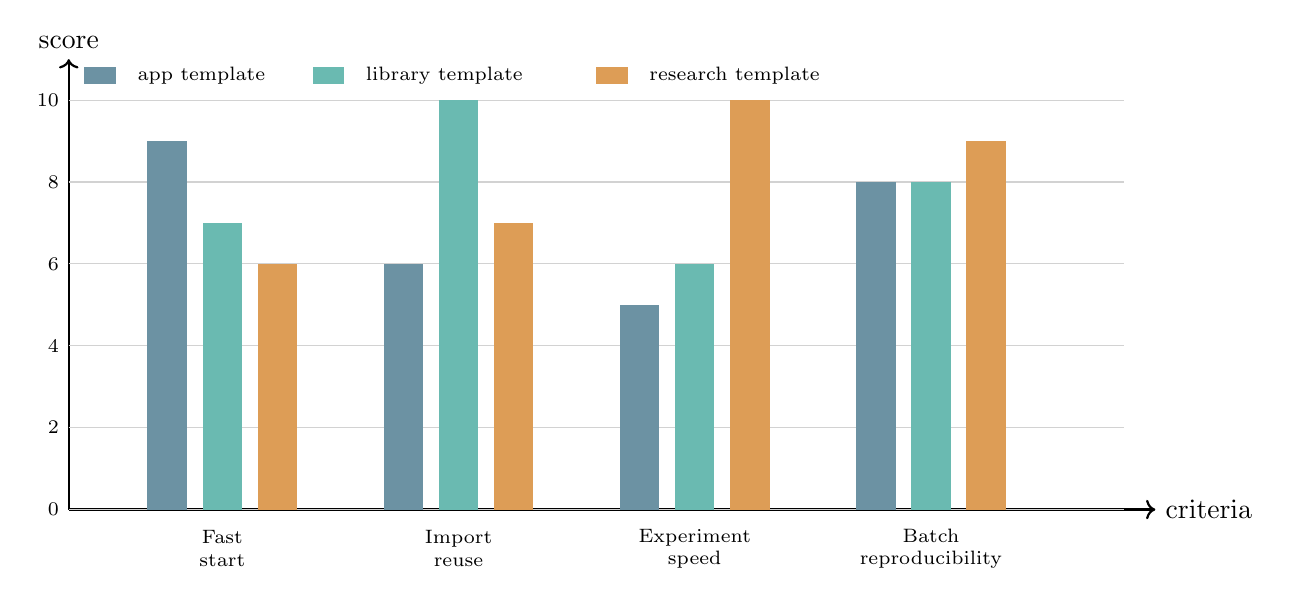
\begin{tikzpicture}[x=1cm,y=0.52cm]
  \draw[->,thick] (0,0) -- (13.8,0) node[right]{criteria};
  \draw[->,thick] (0,0) -- (0,11) node[above]{score};

  \foreach \y in {0,2,4,6,8,10} {
    \draw[gray!35] (0,\y) -- (13.4,\y);
    \node[left,font=\scriptsize] at (0,\y) {\y};
  }

  \fill[bookblue!60] (1.0,0) rectangle (1.5,9);
  \fill[bookteal!70] (1.7,0) rectangle (2.2,7);
  \fill[bookgold!75] (2.4,0) rectangle (2.9,6);

  \fill[bookblue!60] (4.0,0) rectangle (4.5,6);
  \fill[bookteal!70] (4.7,0) rectangle (5.2,10);
  \fill[bookgold!75] (5.4,0) rectangle (5.9,7);

  \fill[bookblue!60] (7.0,0) rectangle (7.5,5);
  \fill[bookteal!70] (7.7,0) rectangle (8.2,6);
  \fill[bookgold!75] (8.4,0) rectangle (8.9,10);

  \fill[bookblue!60] (10.0,0) rectangle (10.5,8);
  \fill[bookteal!70] (10.7,0) rectangle (11.2,8);
  \fill[bookgold!75] (11.4,0) rectangle (11.9,9);

  \node[align=center,font=\scriptsize] at (1.95,-0.95) {Fast\\start};
  \node[align=center,font=\scriptsize] at (4.95,-0.95) {Import\\reuse};
  \node[align=center,font=\scriptsize] at (7.95,-0.95) {Experiment\\speed};
  \node[align=center,font=\scriptsize] at (10.95,-0.95) {Batch\\reproducibility};

  \fill[bookblue!60] (0.2,10.4) rectangle (0.6,10.8);
  \node[anchor=west,font=\scriptsize] at (0.75,10.6) {app template};
  \fill[bookteal!70] (3.1,10.4) rectangle (3.5,10.8);
  \node[anchor=west,font=\scriptsize] at (3.65,10.6) {library template};
  \fill[bookgold!75] (6.7,10.4) rectangle (7.1,10.8);
  \node[anchor=west,font=\scriptsize] at (7.25,10.6) {research template};
\end{tikzpicture}
\caption{Template choice guide for selecting a project family from its constraints.}
\end{figure}

\chapter{Core Root Components}

The example layout has five large structural zones plus a set of root-level policy and setup files.

\section*{What the root zones do}
\begin{itemize}
  \item \texttt{templates/}: copyable starter projects teaching clean project anatomy.
  \item \texttt{examples/}: runnable demonstrations proving the starter patterns actually worked.
  \item \texttt{tools/}: automation helpers, especially the project generator.
  \item \texttt{data/} and \texttt{outputs/}: boundary markers separating source code from mutable local state.
  \item \texttt{notebooks/}: ordered interactive lessons for active practice and recall.
  \item root files: packaging, workflow, security, dependency, and onboarding guidance.
\end{itemize}

\begin{figure}[H]
\centering
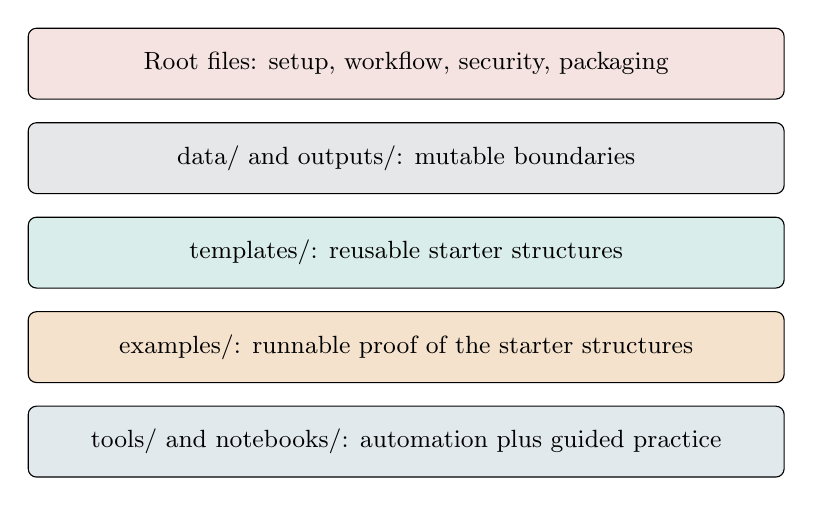
\begin{tikzpicture}[every node/.style={font=\small, align=center}]
  \node[draw, rounded corners=3pt, fill=bookred!16, minimum width=9.6cm, minimum height=0.9cm] (layer1) at (0,2.6) {Root files: setup, workflow, security, packaging};
  \node[draw, rounded corners=3pt, fill=bookgray!14, minimum width=9.6cm, minimum height=0.9cm] (layer2) at (0,1.4) {data/ and outputs/: mutable boundaries};
  \node[draw, rounded corners=3pt, fill=bookteal!18, minimum width=9.6cm, minimum height=0.9cm] (layer3) at (0,0.2) {templates/: reusable starter structures};
  \node[draw, rounded corners=3pt, fill=bookgold!22, minimum width=9.6cm, minimum height=0.9cm] (layer4) at (0,-1.0) {examples/: runnable proof of the starter structures};
  \node[draw, rounded corners=3pt, fill=bookblue!12, minimum width=9.6cm, minimum height=0.9cm] (layer5) at (0,-2.2) {tools/ and notebooks/: automation plus guided practice};
\end{tikzpicture}
\caption{A stack view of a complete project structure: policy at the top, practice at the bottom.}
\end{figure}

\memorybox{
\textbf{Interpretation rule:} if two paths seem similar, ask which one teaches the pattern and which one proves the pattern.  
In this pattern, \texttt{templates/} teach and \texttt{examples/} prove.
}

\section*{The Root Files That Usually Exist}

At the project root, the goal is not to collect random files.  
The goal is to place only the files that coordinate the whole project.

\begin{lstlisting}[style=bookcode]
README.md
pyproject.toml
.gitignore
requirements.txt
requirements-dev.txt
main.py
Makefile
SECURITY.md
TEAM_WORKFLOW.md
\end{lstlisting}

These files belong at the root because they answer repository-wide questions:
\begin{itemize}
  \item \texttt{README.md}: what this project is and how to use it,
  \item \texttt{pyproject.toml}: how packaging and tools are configured,
  \item \texttt{main.py}: where one default run begins,
  \item \texttt{requirements*.txt}: which dependencies are needed,
  \item \texttt{Makefile}: which repeated commands should be memorable,
  \item policy files: how people work safely and consistently.
\end{itemize}

\section*{What Should Not Be At The Root}

The root becomes noisy when every new concern creates another loose file.  
Avoid putting these directly at the top level unless there is a strong reason:
\begin{itemize}
  \item experimental scratch scripts,
  \item ad hoc CSV outputs,
  \item notebook exports,
  \item helper modules that should really live under \texttt{src/},
  \item duplicate configuration files with unclear ownership.
\end{itemize}

\section*{A Reliable Top-Level Map}

\begin{figure}[H]
\centering
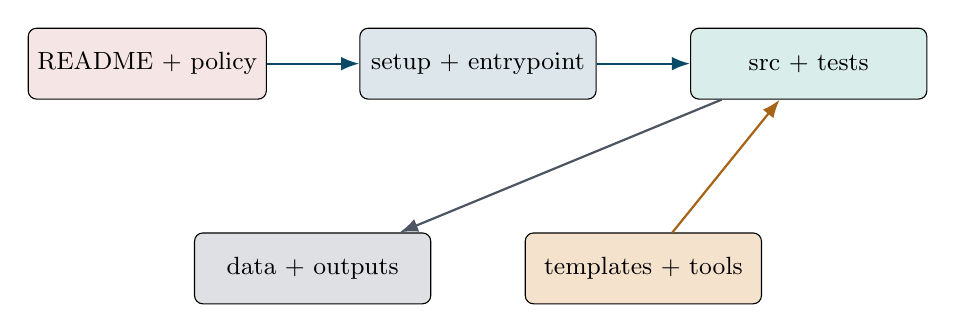
\begin{tikzpicture}[>=Latex, every node/.style={font=\small, align=center}]
  \node[draw, rounded corners=3pt, fill=bookred!14, minimum width=3.0cm, minimum height=0.9cm] (docs) at (-4.2,1.6) {README + policy};
  \node[draw, rounded corners=3pt, fill=bookblue!14, minimum width=3.0cm, minimum height=0.9cm] (setup) at (0,1.6) {setup + entrypoint};
  \node[draw, rounded corners=3pt, fill=bookteal!18, minimum width=3.0cm, minimum height=0.9cm] (code) at (4.2,1.6) {src + tests};
  \node[draw, rounded corners=3pt, fill=bookgray!18, minimum width=3.0cm, minimum height=0.9cm] (state) at (-2.1,-1.0) {data + outputs};
  \node[draw, rounded corners=3pt, fill=bookgold!22, minimum width=3.0cm, minimum height=0.9cm] (support) at (2.1,-1.0) {templates + tools};

  \draw[->, thick, bookblue] (docs) -- (setup);
  \draw[->, thick, bookblue] (setup) -- (code);
  \draw[->, thick, bookgray] (code) -- (state);
  \draw[->, thick, bookgold!80!black] (support) -- (code);
\end{tikzpicture}
\caption{The root stays readable when documentation, setup, code, state, and support layers are visibly separated.}
\end{figure}

\chapter{Building A Readable Project Tree}

This chapter is the practical core of the book.  
Its job is to teach one clean default structure that you can reuse in most Python projects, then explain how the folders, files, and pipeline fit together.

A readable project answers these questions quickly:
\begin{itemize}
  \item Where do I start the program?
  \item Where do I change configuration?
  \item Where does reusable code live?
  \item Where do tests verify behavior?
  \item Where do data and generated files go?
\end{itemize}

\section*{The Minimal Tree To Memorize}

If you remember only one structure from this book, remember this one:

\begin{lstlisting}[style=bookcode]
my_project/
  README.md
  pyproject.toml
  .gitignore
  main.py
  configs/
    config.yaml
  data/
    .gitkeep
  outputs/
    .gitkeep
  src/
    my_project/
      __init__.py
      config.py
      logging_utils.py
      pipeline.py
      steps.py
  tests/
    test_import.py
    test_pipeline_smoke.py
\end{lstlisting}

\memorybox{
\textbf{Memorization rule:} keep orchestration thin at the root, keep reusable code under \texttt{src/}, keep verification under \texttt{tests/}, and keep mutable local state under \texttt{data/} or \texttt{outputs/}.  
That one rule prevents a large share of unreadable projects.
}

\section*{How To Read The Tree}

\begin{figure}[H]
\centering
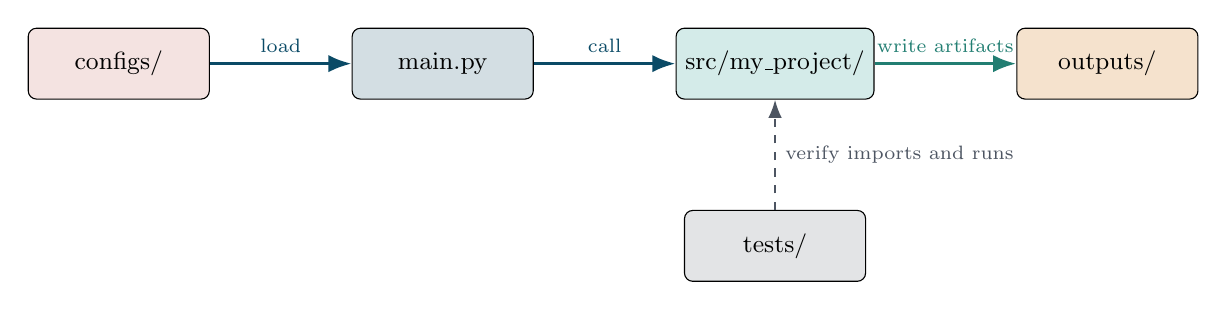
\begin{tikzpicture}[>=Latex, node distance=1.8cm, every node/.style={font=\small}]
  \node[draw, rounded corners=3pt, fill=bookred!16, minimum width=2.3cm, minimum height=0.9cm] (cfg) {configs/};
  \node[draw, rounded corners=3pt, fill=bookblue!18, minimum width=2.3cm, minimum height=0.9cm, right=of cfg] (main) {main.py};
  \node[draw, rounded corners=3pt, fill=bookteal!20, minimum width=2.5cm, minimum height=0.9cm, right=of main] (src) {src/my\_project/};
  \node[draw, rounded corners=3pt, fill=bookgold!22, minimum width=2.3cm, minimum height=0.9cm, right=of src] (out) {outputs/};
  \node[draw, rounded corners=3pt, fill=bookgray!16, minimum width=2.3cm, minimum height=0.9cm, below=1.4cm of src] (tests) {tests/};

  \draw[->, very thick, bookblue] (cfg) -- node[above,font=\scriptsize]{load} (main);
  \draw[->, very thick, bookblue] (main) -- node[above,font=\scriptsize]{call} (src);
  \draw[->, very thick, bookteal!80!black] (src) -- node[above,font=\scriptsize]{write artifacts} (out);
  \draw[->, dashed, thick, bookgray] (tests) -- node[right,font=\scriptsize]{verify imports and runs} (src);
\end{tikzpicture}
\caption{The clean path through a project: configuration enters, code runs, tests verify, artifacts leave source folders.}
\end{figure}

Read this structure from left to right:
\begin{itemize}
  \item \texttt{configs/} answers \textit{with which parameters do we run?}
  \item \texttt{main.py} answers \textit{where does execution start?}
  \item \texttt{src/my\_project/} answers \textit{where does the real logic live?}
  \item \texttt{tests/} answers \textit{how do we know the logic still works?}
  \item \texttt{outputs/} answers \textit{where do generated results go?}
\end{itemize}

\section*{What Each Folder Means}

\subsection*{\texttt{src/}: the home of reusable code}
\texttt{src/} exists to hold code that should be imported, tested, reused, and reviewed.  
If a function matters to the project, it should usually live here instead of being buried inside a notebook or a long root script.

Usually put these files in the package:
\begin{itemize}
  \item \texttt{\_\_init\_\_.py}: defines the public boundary of the package.
  \item \texttt{config.py}: loads and validates configuration.
  \item \texttt{logging\_utils.py}: centralizes log formatting and log levels.
  \item \texttt{pipeline.py}: defines the order of execution.
  \item \texttt{steps.py}: contains the small units of work called by the pipeline.
\end{itemize}

\subsection*{\texttt{tests/}: the proof that the structure works}
\texttt{tests/} must stay close to the behavior users actually depend on.  
For a small project, two tests already teach a lot:
\begin{itemize}
  \item an import smoke test to verify the package surface,
  \item a pipeline smoke test to verify one real run from config to artifact.
\end{itemize}

\subsection*{\texttt{configs/}: run behavior without code edits}
\texttt{configs/} is where you change runtime parameters without editing Python modules.  
This keeps runs reproducible and makes review easier because behavior changes appear as config diffs, not hidden code edits.

\subsection*{\texttt{data/} and \texttt{outputs/}: keep mutable state out of code}
\texttt{data/} is for inputs. \texttt{outputs/} is for artifacts produced by the run.  
The reason is simple: code folders should explain logic, while data and result folders should hold state that changes from run to run.

\subsection*{Root files: thin coordination only}
Root files should stay short and purposeful:
\begin{itemize}
  \item \texttt{README.md}: how to understand and run the project.
  \item \texttt{pyproject.toml}: tool and packaging configuration.
  \item \texttt{.gitignore}: keep clutter out of version control.
  \item \texttt{main.py}: wire the parts together, but do not hide business logic here.
\end{itemize}

\actionbox{
\textbf{Anti-pattern to avoid}  
If \texttt{main.py} becomes a 400-line script that loads YAML, performs all transformations, writes files, and prints metrics, the project has no reusable center.  
Move that logic under \texttt{src/} and let \texttt{main.py} remain a thin entrypoint.
}

\section*{Code Explanation: A Thin \texttt{main.py}}

\begin{lstlisting}[style=bookcode,language=Python]
from my_project.config import load_config
from my_project.logging_utils import configure_logging
from my_project.pipeline import build_pipeline, run_pipeline


def main() -> None:
    config = load_config("configs/config.yaml")
    configure_logging(config.log_level)
    pipeline = build_pipeline(config)
    run_pipeline(pipeline, config)


if __name__ == "__main__":
    main()
\end{lstlisting}

Why this is good:
\begin{itemize}
  \item It starts the application in one obvious place.
  \item It loads configuration instead of hard-coding values.
  \item It delegates real work to importable modules under \texttt{src/}.
  \item It stays short enough that a reader can understand the execution path in seconds.
\end{itemize}

\section*{Code Explanation: A Clear \texttt{config.py}}

\begin{lstlisting}[style=bookcode,language=Python]
from dataclasses import dataclass
from pathlib import Path

import yaml


@dataclass
class AppConfig:
    run_name: str
    output_dir: Path
    log_level: str = "INFO"


def load_config(path: str) -> AppConfig:
    raw = yaml.safe_load(Path(path).read_text())
    return AppConfig(
        run_name=raw["run_name"],
        output_dir=Path(raw["output_dir"]),
        log_level=raw.get("log_level", "INFO"),
    )
\end{lstlisting}

What this file teaches:
\begin{itemize}
  \item configuration becomes a typed object, not a loose dictionary passed everywhere,
  \item defaults are applied in one place,
  \item path conversion happens once instead of being repeated across the codebase.
\end{itemize}

The matching YAML can stay very simple:

\begin{lstlisting}[style=bookcode,language=yaml]
run_name: demo_run
output_dir: outputs/demo_run
log_level: INFO
\end{lstlisting}

\section*{Code Explanation: \texttt{pipeline.py} Owns Order}

\begin{lstlisting}[style=bookcode,language=Python]
from dataclasses import dataclass, field
from pathlib import Path
from typing import Callable

from my_project.config import AppConfig

Step = Callable[["PipelineContext"], None]


@dataclass
class PipelineContext:
    config: AppConfig
    artifacts: dict[str, Path] = field(default_factory=dict)
    metrics: dict[str, float] = field(default_factory=dict)


def build_pipeline(config: AppConfig) -> list[Step]:
    from my_project.steps import compute_total, write_report

    return [compute_total, write_report]


def run_pipeline(steps: list[Step], config: AppConfig) -> PipelineContext:
    context = PipelineContext(config=config)
    for step in steps:
        step(context)
    return context
\end{lstlisting}

Why this separation matters:
\begin{itemize}
  \item \texttt{pipeline.py} explains order and shared context.
  \item \texttt{steps.py} stays focused on small units of behavior.
  \item adding a new step becomes a one-line change in the pipeline instead of a rewrite of the whole program.
\end{itemize}

\section*{Code Explanation: \texttt{steps.py} Owns Work Units}

\begin{lstlisting}[style=bookcode,language=Python]
from pathlib import Path

from my_project.pipeline import PipelineContext


def compute_total(context: PipelineContext) -> None:
    values = [2, 5, 9]
    total = sum(values)
    context.metrics["total"] = float(total)
    context.artifacts["summary"] = context.config.output_dir / "summary.txt"


def write_report(context: PipelineContext) -> None:
    report_path = context.artifacts["summary"]
    report_path.parent.mkdir(parents=True, exist_ok=True)
    report_path.write_text(f"total={context.metrics['total']}\n")
\end{lstlisting}

This is the pattern to keep:
\begin{itemize}
  \item each step has one job,
  \item the step reads from shared context instead of guessing global state,
  \item generated files are written into \texttt{outputs/}, never into \texttt{src/}.
\end{itemize}

\section*{Code Explanation: \texttt{\_\_init\_\_.py} Defines The Public API}

\begin{lstlisting}[style=bookcode,language=Python]
from my_project.config import AppConfig, load_config
from my_project.pipeline import build_pipeline, run_pipeline

__all__ = ["AppConfig", "build_pipeline", "load_config", "run_pipeline"]
\end{lstlisting}

This file tells readers which names are meant to be imported from the package directly.  
Without this boundary, internal helpers leak into public usage and refactoring becomes harder.

\section*{How The Structure Changes By Project Type}

The basic tree stays the same, but the emphasis changes:
\begin{itemize}
  \item \textbf{Application project:} keep \texttt{main.py} and \texttt{pipeline.py} central because execution flow is the main product.
  \item \textbf{Library project:} add a clear \texttt{api.py} and keep the public interface small because import reuse is the main product.
  \item \textbf{Research project:} add \texttt{notebooks/} and possibly \texttt{research\_helpers.py}, but still move repeated logic back into \texttt{src/}.
\end{itemize}

\memorybox{
\textbf{Final rule for Chapter 4:} a good structure is readable before you open the code.  
The folder names explain responsibilities, and the code files explain only one layer each: entrypoint, config, pipeline, steps, tests.
}

\chapter{Writing The Key Files}

Chapter 4 taught the folder structure.  
This chapter teaches what should actually be written in the most important files so the project stays readable, reviewable, and reusable.

\section*{One File, One Responsibility}

The fastest way to destroy readability is to let files become mixed-purpose containers.  
Each important file should answer one clear question:
\begin{itemize}
  \item \texttt{README.md}: what is this project and how do I use it?
  \item \texttt{pyproject.toml}: how is this project built and tooled?
  \item \texttt{main.py}: where does execution start?
  \item \texttt{config.py}: how are runtime parameters loaded and shaped?
  \item \texttt{pipeline.py}: in what order do steps run?
  \item \texttt{steps.py}: what does each unit of work do?
  \item \texttt{tests/}: what behavior do we verify automatically?
\end{itemize}

\begin{figure}[H]
\centering
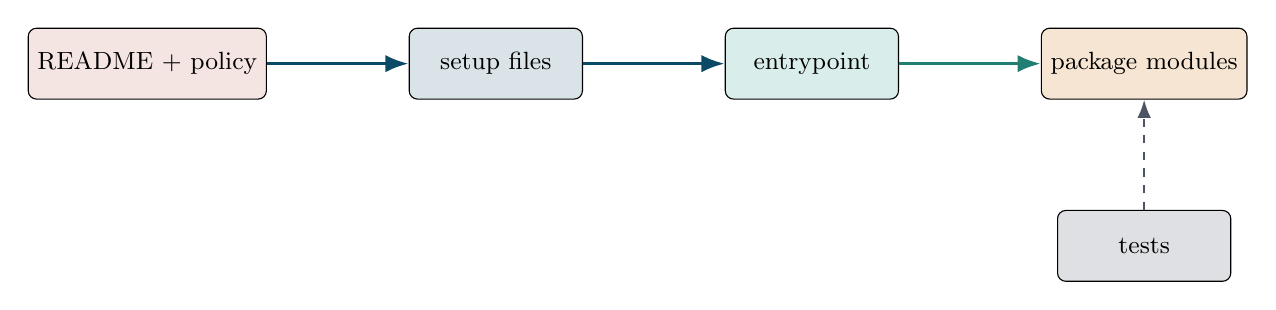
\begin{tikzpicture}[>=Latex, node distance=1.8cm, every node/.style={font=\small}]
  \node[draw, rounded corners=3pt, fill=bookred!15, minimum width=2.5cm, minimum height=0.9cm] (docs) {README + policy};
  \node[draw, rounded corners=3pt, fill=bookblue!15, minimum width=2.2cm, minimum height=0.9cm, right=of docs] (setup) {setup files};
  \node[draw, rounded corners=3pt, fill=bookteal!18, minimum width=2.2cm, minimum height=0.9cm, right=of setup] (run) {entrypoint};
  \node[draw, rounded corners=3pt, fill=bookgold!20, minimum width=2.5cm, minimum height=0.9cm, right=of run] (pkg) {package modules};
  \node[draw, rounded corners=3pt, fill=bookgray!18, minimum width=2.2cm, minimum height=0.9cm, below=1.4cm of pkg] (tests) {tests};

  \draw[->, very thick, bookblue] (docs) -- (setup);
  \draw[->, very thick, bookblue] (setup) -- (run);
  \draw[->, very thick, bookteal!80!black] (run) -- (pkg);
  \draw[->, dashed, thick, bookgray] (tests) -- (pkg);
\end{tikzpicture}
\caption{A readable project moves from orientation files to execution files to reusable modules, with tests checking the modules.}
\end{figure}

\section*{\texttt{README.md}: the front door}

A new reader should learn four things from the README:
\begin{itemize}
  \item what the project does,
  \item how to run it,
  \item what the important folders are,
  \item where to look next.
\end{itemize}

\begin{lstlisting}[style=bookcode]
# My Project

Short purpose sentence.

## Quick Start

python -m venv .venv
source .venv/bin/activate
pip install -r requirements-dev.txt
python main.py

## Project Structure

- configs/: runtime configuration
- src/my_project/: reusable code
- tests/: automated checks
- outputs/: generated artifacts

## Typical Workflow

1. Edit config
2. Run main.py
3. Inspect outputs
4. Run tests
\end{lstlisting}

What usually belongs here:
\begin{itemize}
  \item a short purpose statement,
  \item setup commands that actually work,
  \item one example run command,
  \item a short project map.
\end{itemize}

What should not live here:
\begin{itemize}
  \item internal design history nobody needs on day one,
  \item dozens of stale commands,
  \item explanations that belong in dedicated guide files.
\end{itemize}

\section*{\texttt{.gitignore}: protect repository signal}

\texttt{.gitignore} exists to keep local noise out of version control.  
If this file is weak, the repository fills with cache files, virtual environments, temporary artifacts, and editor clutter.

\begin{lstlisting}[style=bookcode]
__pycache__/
.pytest_cache/
.venv/
.mypy_cache/
outputs/
*.log
.DS_Store
\end{lstlisting}

Good ignore rules do three things:
\begin{itemize}
  \item ignore machine-specific noise,
  \item ignore generated local artifacts,
  \item keep source and intentional configuration visible.
\end{itemize}

\section*{\texttt{pyproject.toml}: the tool contract}

This file is the center of build and tool configuration.  
It should give the project one clear home for packaging and developer-tool settings.

\begin{lstlisting}[style=bookcode]
[build-system]
requires = ["setuptools>=68", "wheel"]
build-backend = "setuptools.build_meta"

[project]
name = "my-project"
version = "0.1.0"
requires-python = ">=3.11"

[tool.pytest.ini_options]
testpaths = ["tests"]

[tool.ruff]
line-length = 100
\end{lstlisting}

Why this matters:
\begin{itemize}
  \item tooling is discoverable in one place,
  \item new contributors do not need to guess which config files matter,
  \item package metadata and test configuration stay near each other.
\end{itemize}

\section*{\texttt{requirements.txt} and \texttt{requirements-dev.txt}}

Use the two dependency files for different audiences:
\begin{itemize}
  \item \texttt{requirements.txt}: only what the project needs to run.
  \item \texttt{requirements-dev.txt}: runtime requirements plus test, lint, and formatting tools.
\end{itemize}

A clean split keeps production dependencies smaller and local development easier.

\begin{lstlisting}[style=bookcode]
# requirements.txt
PyYAML>=6.0

# requirements-dev.txt
-r requirements.txt
pytest>=8.0
ruff>=0.6
black>=24.0
\end{lstlisting}

\section*{\texttt{main.py}: start, do not own everything}

Chapter 4 already showed a thin \texttt{main.py}.  
The rule is worth repeating: this file should wire together the program, not become the whole program.

What usually belongs in \texttt{main.py}:
\begin{itemize}
  \item CLI or path selection,
  \item config loading,
  \item logging setup,
  \item one call into the pipeline or public API.
\end{itemize}

What should move out of it:
\begin{itemize}
  \item data transformation logic,
  \item repeated helper functions,
  \item direct business rules,
  \item testable units of behavior.
\end{itemize}

\section*{\texttt{logging\_utils.py}: one voice for the whole project}

Logging becomes unreadable when each file invents its own format.  
Keep logging setup in one module so every run speaks in the same style.

\begin{lstlisting}[style=bookcode,language=Python]
import logging


def configure_logging(level: str = "INFO") -> None:
    logging.basicConfig(
        level=getattr(logging, level.upper(), logging.INFO),
        format="%(asctime)s | %(levelname)s | %(name)s | %(message)s",
    )
\end{lstlisting}

This file should usually:
\begin{itemize}
  \item define the base log format,
  \item convert string log levels into logging constants,
  \item centralize logging decisions instead of repeating them across modules.
\end{itemize}

\section*{\texttt{\_\_init\_\_.py} and \texttt{api.py}: public boundaries}

For application projects, \texttt{\_\_init\_\_.py} often exports only a small public surface.  
For library projects, add an \texttt{api.py} file when you want downstream users to import reusable functions directly.

\begin{lstlisting}[style=bookcode,language=Python]
# api.py
def normalize_name(value: str) -> str:
    return value.strip().title()


# __init__.py
from my_project.api import normalize_name

__all__ = ["normalize_name"]
\end{lstlisting}

This is important because:
\begin{itemize}
  \item consumers need a stable import path,
  \item internal helpers should stay internal,
  \item refactoring becomes safer when the public surface is explicit.
\end{itemize}

\section*{\texttt{tests/test\_import.py}: the fastest useful test}

The import smoke test verifies that the public package surface still exists and can be imported.  
It is small, fast, and catches surprisingly common breakage.

\begin{lstlisting}[style=bookcode,language=Python]
from my_project import build_pipeline, load_config, run_pipeline


def test_public_imports() -> None:
    assert callable(load_config)
    assert callable(build_pipeline)
    assert callable(run_pipeline)
\end{lstlisting}

This test is not deep, but it is valuable because it protects the first thing users rely on: imports.

\section*{\texttt{tests/test\_pipeline\_smoke.py}: one real execution}

If the project has a pipeline, one smoke test should run the smallest realistic path from configuration to output.

\begin{lstlisting}[style=bookcode,language=Python]
from pathlib import Path

from my_project.config import AppConfig
from my_project.pipeline import build_pipeline, run_pipeline


def test_pipeline_smoke(tmp_path: Path) -> None:
    config = AppConfig(
        run_name="test_run",
        output_dir=tmp_path / "outputs",
        log_level="INFO",
    )
    context = run_pipeline(build_pipeline(config), config)
    assert "summary" in context.artifacts
    assert context.artifacts["summary"].exists()
\end{lstlisting}

What this test teaches:
\begin{itemize}
  \item the modules connect correctly,
  \item the pipeline produces a real artifact,
  \item the output boundary is honored.
\end{itemize}

\section*{\texttt{Makefile}: memorable commands for humans}

A \texttt{Makefile} is useful when it shortens repeated commands and reduces setup mistakes.

\begin{lstlisting}[style=bookcode]
setup:
	python -m venv .venv
	. .venv/bin/activate && pip install -r requirements-dev.txt

run:
	python main.py

test:
	pytest
\end{lstlisting}

Keep it simple.  
It should improve memory and consistency, not hide mysterious behavior behind vague target names.

\section*{Policy Files: make collaboration explicit}

Not every important file is code.  
Some files keep team behavior readable:
\begin{itemize}
  \item \texttt{TEAM\_WORKFLOW.md}: branching, review rules, commit expectations, release flow.
  \item \texttt{SECURITY.md}: secret handling, reporting process, dependency caution.
  \item \texttt{PROJECT\_STRUCTURE\_GUIDE.md}: why the tree is organized this way.
  \item \texttt{PIPELINE\_STYLE\_GUIDE.md}: how config, steps, logs, metrics, and artifacts should interact.
\end{itemize}

These files matter because a project can be structurally clean and still be difficult to work with if team rules remain implicit.

\section*{Optional Files By Project Type}

Some files appear only when the project needs them:
\begin{itemize}
  \item \textbf{Research project:} add \texttt{notebooks/} and maybe \texttt{research\_helpers.py}.
  \item \textbf{Library project:} add \texttt{api.py} to expose reusable functions.
  \item \textbf{Template repository:} add \texttt{tools/new\_project.py} to scaffold new instances of the structure.
\end{itemize}

Only add these files when they solve a real problem.  
Optional files are powerful, but unnecessary files add noise quickly.

\actionbox{
\textbf{File quality checklist}
\begin{itemize}
  \item Can you explain why this file exists in one sentence?
  \item Does it own one layer of responsibility?
  \item Would a new contributor know when to open it?
  \item If the file disappeared, would the project lose a clear capability?
\end{itemize}
}

\chapter{Designing A Reliable Pipeline}

Project structure is not complete until one run can move through the code in a traceable way.  
This chapter explains how configuration, steps, logs, metrics, and artifacts should behave together.

\section*{The Lifecycle Of One Run}

\begin{figure}[H]
\centering
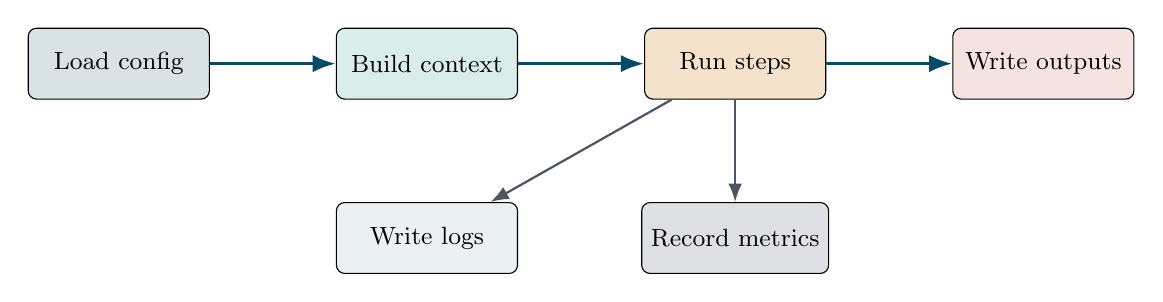
\begin{tikzpicture}[>=Latex, node distance=1.6cm, every node/.style={font=\small}]
  \node[draw, rounded corners=3pt, fill=bookblue!16, minimum width=2.3cm, minimum height=0.9cm] (cfg) {Load config};
  \node[draw, rounded corners=3pt, fill=bookteal!18, minimum width=2.3cm, minimum height=0.9cm, right=of cfg] (ctx) {Build context};
  \node[draw, rounded corners=3pt, fill=bookgold!22, minimum width=2.3cm, minimum height=0.9cm, right=of ctx] (steps) {Run steps};
  \node[draw, rounded corners=3pt, fill=bookred!16, minimum width=2.3cm, minimum height=0.9cm, right=of steps] (art) {Write outputs};
  \node[draw, rounded corners=3pt, fill=bookgray!18, minimum width=2.3cm, minimum height=0.9cm, below=1.3cm of steps] (met) {Record metrics};
  \node[draw, rounded corners=3pt, fill=bookblue!8, minimum width=2.3cm, minimum height=0.9cm, below=1.3cm of ctx] (log) {Write logs};

  \draw[->, very thick, bookblue] (cfg) -- (ctx);
  \draw[->, very thick, bookblue] (ctx) -- (steps);
  \draw[->, very thick, bookblue] (steps) -- (art);
  \draw[->, thick, bookgray] (steps) -- (met);
  \draw[->, thick, bookgray] (steps) -- (log);
\end{tikzpicture}
\caption{A reliable run follows one visible path: config, context, steps, outputs, logs, and metrics.}
\end{figure}

\section*{What Configuration Should Control}

Configuration should describe variation between runs, not replace code design.  
Good configuration usually contains:
\begin{itemize}
  \item input and output paths,
  \item run names,
  \item log levels,
  \item numerical thresholds or feature toggles,
  \item selected modes that the code already knows how to handle.
\end{itemize}

Good configuration usually should not contain:
\begin{itemize}
  \item raw Python expressions,
  \item hidden business logic,
  \item values loaded from many unrelated files without explanation.
\end{itemize}

\begin{lstlisting}[style=bookcode,language=yaml]
run_name: train_small
input_path: data/input.csv
output_dir: outputs/train_small
log_level: INFO
threshold: 0.8
mode: baseline
\end{lstlisting}

\section*{What The Pipeline Context Should Carry}

The context object is the shared state of one run.  
It should carry only the information that steps need to coordinate safely.

\begin{lstlisting}[style=bookcode,language=Python]
from dataclasses import dataclass, field
from pathlib import Path


@dataclass
class PipelineContext:
    config: AppConfig
    run_dir: Path
    artifacts: dict[str, Path] = field(default_factory=dict)
    metrics: dict[str, float] = field(default_factory=dict)
    notes: list[str] = field(default_factory=list)
\end{lstlisting}

This pattern helps because:
\begin{itemize}
  \item steps do not need hidden globals,
  \item the run has one explicit place for produced paths,
  \item debugging becomes easier because shared state is inspectable.
\end{itemize}

\section*{What A Good Step Looks Like}

A good step is small enough to describe in one sentence.  
It reads from context, performs one responsibility, and writes explicit outputs back to context.

\begin{lstlisting}[style=bookcode,language=Python]
def clean_records(context: PipelineContext) -> None:
    input_path = Path(context.config.input_path)
    output_path = context.run_dir / "clean_records.csv"

    rows = [line.strip() for line in input_path.read_text().splitlines() if line.strip()]
    cleaned = [row.lower() for row in rows]

    output_path.write_text("\n".join(cleaned) + "\n")
    context.artifacts["clean_records"] = output_path
    context.metrics["record_count"] = float(len(cleaned))
\end{lstlisting}

This step is readable because:
\begin{itemize}
  \item inputs are obvious,
  \item the produced file is explicit,
  \item metrics are recorded at the place they are created.
\end{itemize}

\section*{Artifacts, Logs, And Metrics Are Different Things}

These three are often mixed together, but they play different roles:
\begin{itemize}
  \item \textbf{Artifacts:} files created by the run, such as reports, CSVs, images, or models.
  \item \textbf{Logs:} chronological messages that explain what happened during execution.
  \item \textbf{Metrics:} structured numbers used for comparison, validation, or monitoring.
\end{itemize}

Keep them separate because each serves a different debugging question:
\begin{itemize}
  \item artifact question: \textit{what was produced?}
  \item log question: \textit{what happened during execution?}
  \item metric question: \textit{how good was the result?}
\end{itemize}

\section*{How To Name Run Outputs}

Output names should make runs traceable without opening the files.

\begin{lstlisting}[style=bookcode]
outputs/
  train_small/
    clean_records.csv
    summary.txt
    metrics.json
    run.log
\end{lstlisting}

This layout is better than scattering files because it keeps one run together.  
If the project produces multiple runs, each run should usually get its own directory.

\section*{How To Handle Failure Without Losing Traceability}

Reliable pipelines fail in visible ways.  
That means:
\begin{itemize}
  \item create the run directory early,
  \item write logs from the beginning of execution,
  \item keep step names explicit in messages,
  \item avoid deleting partial outputs automatically unless corruption is guaranteed.
\end{itemize}

\begin{lstlisting}[style=bookcode,language=Python]
def run_pipeline(steps: list[Step], config: AppConfig) -> PipelineContext:
    run_dir = config.output_dir
    run_dir.mkdir(parents=True, exist_ok=True)
    context = PipelineContext(config=config, run_dir=run_dir)

    for step in steps:
        step(context)

    return context
\end{lstlisting}

\section*{Common Pipeline Anti-Patterns}

\begin{itemize}
  \item loading configuration separately inside many steps,
  \item writing outputs into \texttt{src/} or beside source modules,
  \item using global variables for shared run state,
  \item putting five unrelated transformations into one giant step,
  \item treating notebooks as the only executable source of truth.
\end{itemize}

\memorybox{
\textbf{Pipeline rule:} one run should be explainable as a path, not as a mystery.  
If you cannot draw the flow from config to outputs on paper, the implementation is probably too entangled.
}

\chapter{Choosing The Right Project Shape}

Not every project should have identical top-level details.  
The right shape depends on the main product the repository is trying to deliver.

\section*{Application Shape}

Choose an application structure when the main value of the project is one executable flow.

\begin{lstlisting}[style=bookcode]
app_project/
  README.md
  main.py
  configs/
  src/app_project/
    __init__.py
    config.py
    pipeline.py
    steps.py
  tests/
\end{lstlisting}

Good fit:
\begin{itemize}
  \item batch jobs,
  \item command-line tools,
  \item scheduled processing pipelines,
  \item internal automation scripts that became real software.
\end{itemize}

\section*{Library Shape}

Choose a library structure when the main value is import reuse by other code.

\begin{lstlisting}[style=bookcode]
library_project/
  README.md
  pyproject.toml
  src/library_project/
    __init__.py
    api.py
    validators.py
    transforms.py
  tests/
\end{lstlisting}

Good fit:
\begin{itemize}
  \item reusable utilities,
  \item business-rule packages,
  \item internal SDKs,
  \item shared transformation or validation logic.
\end{itemize}

Key rule: the public API must stay smaller than the internal implementation.

\section*{Research Shape}

Choose a research structure when exploration is necessary but reproducible code still matters.

\begin{lstlisting}[style=bookcode]
research_project/
  README.md
  main.py
  configs/
  notebooks/
  src/research_project/
    __init__.py
    config.py
    pipeline.py
    research_helpers.py
  tests/
  outputs/
\end{lstlisting}

Good fit:
\begin{itemize}
  \item experiments with many iterations,
  \item model comparisons,
  \item exploratory analysis that must eventually become reproducible.
\end{itemize}

Key rule: notebooks may explore, but repeated logic must migrate back into \texttt{src/}.

\section*{When To Upgrade From One Shape To Another}

Projects often evolve:
\begin{itemize}
  \item an application grows a small \texttt{api.py} when other services need its logic,
  \item a research repository becomes an application once experiments stabilize into one main run,
  \item a library project gains a tiny \texttt{main.py} when maintainers want a smoke-run command.
\end{itemize}

Changing shape is normal.  
What matters is that the structure reflects the dominant usage mode clearly.

\section*{A Quick Decision Guide}

\begin{itemize}
  \item If users mostly run one command: start with an application structure.
  \item If users mostly import functions: start with a library structure.
  \item If users mostly explore hypotheses: start with a research structure.
\end{itemize}

\begin{figure}[H]
\centering
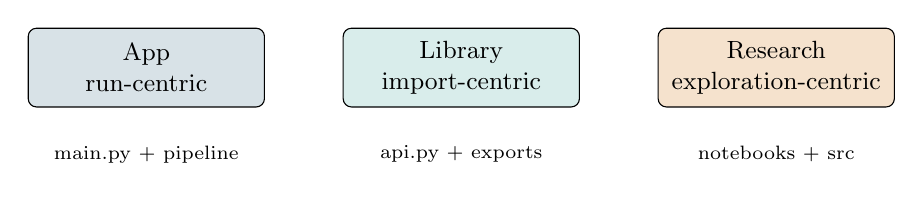
\begin{tikzpicture}[>=Latex, every node/.style={font=\small, align=center}]
  \node[draw, rounded corners=3pt, fill=bookblue!16, minimum width=3.0cm, minimum height=1.0cm] (app) at (-4.0,0) {App\\run-centric};
  \node[draw, rounded corners=3pt, fill=bookteal!18, minimum width=3.0cm, minimum height=1.0cm] (lib) at (0,0) {Library\\import-centric};
  \node[draw, rounded corners=3pt, fill=bookgold!22, minimum width=3.0cm, minimum height=1.0cm] (res) at (4.0,0) {Research\\exploration-centric};

  \node[font=\scriptsize] at (-4.0,-1.1) {main.py + pipeline};
  \node[font=\scriptsize] at (0,-1.1) {api.py + exports};
  \node[font=\scriptsize] at (4.0,-1.1) {notebooks + src};
\end{tikzpicture}
\caption{Choose the shape that matches the primary way the project is consumed.}
\end{figure}

\chapter{Building A Project From Zero}

This chapter turns the book into a practical workflow.  
If you start with an empty directory, the steps below are enough to build a clean project skeleton without guessing.

\section*{Step 1: Create The Root Skeleton}

\begin{lstlisting}[style=bookcode]
mkdir -p my_project/configs my_project/data my_project/outputs
mkdir -p my_project/src/my_project my_project/tests
\end{lstlisting}

Then add the minimum root files:
\begin{lstlisting}[style=bookcode]
README.md
pyproject.toml
.gitignore
main.py
requirements.txt
requirements-dev.txt
\end{lstlisting}

\section*{Step 2: Create The Package Core}

Start with five modules under \texttt{src/my\_project/}:
\begin{itemize}
  \item \texttt{\_\_init\_\_.py}
  \item \texttt{config.py}
  \item \texttt{logging\_utils.py}
  \item \texttt{pipeline.py}
  \item \texttt{steps.py}
\end{itemize}

This is enough for a first clean version.  
Do not create extra modules until you can name their responsibility clearly.

\section*{Step 3: Add One Config And One Run Path}

Write one config file and make one happy-path run work first.

\begin{lstlisting}[style=bookcode,language=yaml]
run_name: first_run
output_dir: outputs/first_run
log_level: INFO
\end{lstlisting}

Early projects often fail because they try to support many modes before one basic path is reliable.

\section*{Step 4: Add Two Tests Immediately}

The first useful tests are still the same:
\begin{itemize}
  \item import smoke test,
  \item pipeline smoke test.
\end{itemize}

This gives you an early warning system before the project grows.

\section*{Step 5: Run, Inspect, Refactor Once}

After the first successful run:
\begin{itemize}
  \item inspect the output directory,
  \item inspect the logs,
  \item remove duplicated code from \texttt{main.py},
  \item rename weakly named files before they become permanent.
\end{itemize}

\section*{Step 6: Add Only The Next Necessary Layer}

After the first clean run, choose only the next justified addition:
\begin{itemize}
  \item add \texttt{api.py} if reuse by import matters,
  \item add \texttt{notebooks/} if exploration matters,
  \item add \texttt{tools/} if scaffolding or repeated automation matters,
  \item add policy guides if more than one contributor is involved.
\end{itemize}

\actionbox{
\textbf{Build-from-zero rule}
\begin{itemize}
  \item Do not start with a huge tree.
  \item Start with one clean run.
  \item Add structure only when a responsibility becomes real.
\end{itemize}
}

\chapter{Growing Without Losing Readability}

Treat the layout in this book as a menu of good design decisions, not as a rigid law.  
The right structure depends on your constraints:
\begin{itemize}
  \item choose the smallest structure that still keeps responsibilities clear,
  \item keep mutable state out of source folders by separating \texttt{data/} and \texttt{outputs/},
  \item use an app layout when orchestration is central, a library layout when import reuse is central, and a research layout when exploration is central,
  \item move repeated notebook logic into modules under \texttt{src/},
  \item keep root files purposeful: each one should reduce confusion for contributors or users.
\end{itemize}

\section*{When To Split A Module}

Split a module when at least one of these becomes true:
\begin{itemize}
  \item the file now owns more than one responsibility,
  \item readers must scroll through unrelated logic to find one function,
  \item testing one behavior requires importing many others,
  \item the name of the file stopped describing all its contents honestly.
\end{itemize}

\section*{When To Add A Subpackage}

Add a subpackage when several modules belong to one larger concern.  
Examples:
\begin{itemize}
  \item \texttt{io/} for readers and writers,
  \item \texttt{features/} for feature engineering logic,
  \item \texttt{models/} for model wrappers and evaluation helpers.
\end{itemize}

Do not add subpackages just to make the tree look sophisticated.

\section*{How To Keep Notebooks Honest}

Notebooks are useful for exploration, demonstration, and teaching, but they should not become the only source of important logic.

Use this rule:
\begin{itemize}
  \item if the code is repeated, move it into \texttt{src/},
  \item if the notebook explains a concept, keep the explanation in the notebook,
  \item if the notebook produces durable results, write those results into \texttt{outputs/}.
\end{itemize}

\section*{How To Introduce More Tooling Safely}

As a project grows, it may need more tooling:
\begin{itemize}
  \item add linting when style drift starts costing review time,
  \item add formatting when diffs become noisy,
  \item add CI when manual test discipline becomes unreliable,
  \item add release automation only after the public surface is stable.
\end{itemize}

Tooling should clarify the project, not overshadow it.

\section*{Memory Loop}
\begin{figure}[H]
\centering
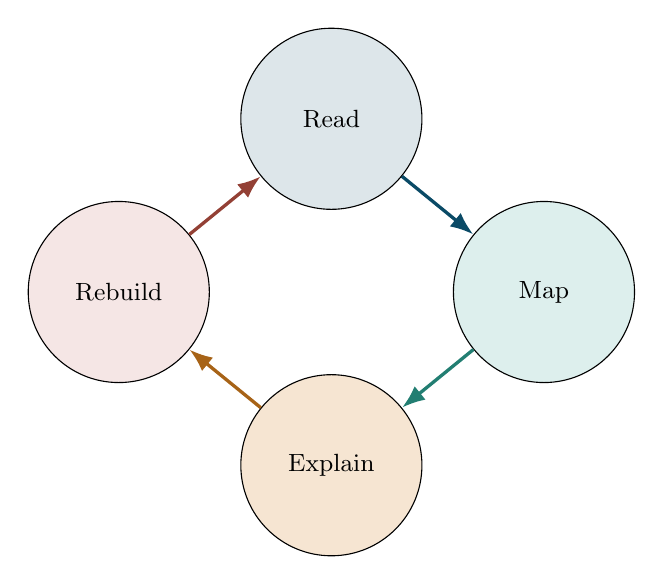
\begin{tikzpicture}[>=Latex, every node/.style={font=\small}]
  \node[draw, circle, fill=bookblue!14, minimum size=2.3cm] (read) at (0,2.2) {Read};
  \node[draw, circle, fill=bookteal!16, minimum size=2.3cm] (map) at (2.7,0) {Map};
  \node[draw, circle, fill=bookgold!20, minimum size=2.3cm] (explain) at (0,-2.2) {Explain};
  \node[draw, circle, fill=bookred!14, minimum size=2.3cm] (rebuild) at (-2.7,0) {Rebuild};

  \draw[->, very thick, bookblue] (read) -- (map);
  \draw[->, very thick, bookteal!80!black] (map) -- (explain);
  \draw[->, very thick, bookgold!80!black] (explain) -- (rebuild);
  \draw[->, very thick, bookred!80!black] (rebuild) -- (read);
\end{tikzpicture}
\caption{Use the book actively: map the structure, explain it, and then rebuild it in your own project.}
\end{figure}

\chapter{Project Review Checklist}

Use this checklist when creating or auditing a project structure:

\actionbox{
\textbf{Review questions}
\begin{itemize}
  \item Can you explain every top-level path in one sentence?
  \item Is there a clear entrypoint for the main way the project is used?
  \item Are config, logs, artifacts, and metrics separated cleanly?
  \item Is repeated notebook or script logic extracted into reusable modules?
  \item Does the public API boundary stay small and intentional?
  \item Can a new contributor find setup, usage, and workflow rules quickly?
\end{itemize}
}

\section*{Root-Level Review}

\begin{itemize}
  \item Are there any root files that should really be inside \texttt{src/}, \texttt{configs/}, or \texttt{outputs/}?
  \item Does each top-level folder have a distinct job?
  \item Are policy files present when the project has team or security needs?
\end{itemize}

\section*{Code-Level Review}

\begin{itemize}
  \item Is \texttt{main.py} still thin?
  \item Are reusable functions in package modules rather than notebooks or loose scripts?
  \item Does each module name match its responsibility?
\end{itemize}

\section*{Pipeline Review}

\begin{itemize}
  \item Can one run be explained from config to artifact in a few sentences?
  \item Are outputs written to run-specific directories?
  \item Are logs and metrics separate from produced artifacts?
\end{itemize}

\section*{Testing Review}

\begin{itemize}
  \item Do the tests verify the public imports?
  \item Does at least one smoke test run a realistic path?
  \item Are tests named after behavior rather than implementation trivia?
\end{itemize}

\section*{Collaboration Review}

\begin{itemize}
  \item Can a new contributor install, run, and test the project from the README?
  \item Are branch, review, and release expectations documented if the project is shared?
  \item Are secrets, local data, and outputs kept out of version control?
\end{itemize}

The structure is usually healthy when:
\begin{itemize}
  \item every folder has one clear responsibility,
  \item every file has a reason to exist,
  \item repeated patterns are documented and reusable,
  \item the project remains understandable without tribal knowledge.
\end{itemize}

\end{document}
